% Options for packages loaded elsewhere
\PassOptionsToPackage{unicode}{hyperref}
\PassOptionsToPackage{hyphens}{url}
%
\documentclass[
  ignorenonframetext,
  serif,
  professionalfont,
  usenames,
  dvipsnames,
  aspectratio = 169]{beamer}
\usepackage{pgfpages}
\setbeamertemplate{caption}[numbered]
\setbeamertemplate{caption label separator}{: }
\setbeamercolor{caption name}{fg=normal text.fg}
\beamertemplatenavigationsymbolsempty
% Prevent slide breaks in the middle of a paragraph
\widowpenalties 1 10000
\raggedbottom
\setbeamertemplate{part page}{
  \centering
  \begin{beamercolorbox}[sep=16pt,center]{part title}
    \usebeamerfont{part title}\insertpart\par
  \end{beamercolorbox}
}
\setbeamertemplate{section page}{
  \centering
  \begin{beamercolorbox}[sep=12pt,center]{part title}
    \usebeamerfont{section title}\insertsection\par
  \end{beamercolorbox}
}
\setbeamertemplate{subsection page}{
  \centering
  \begin{beamercolorbox}[sep=8pt,center]{part title}
    \usebeamerfont{subsection title}\insertsubsection\par
  \end{beamercolorbox}
}
\AtBeginPart{
  \frame{\partpage}
}
\AtBeginSection{
  \ifbibliography
  \else
    \frame{\sectionpage}
  \fi
}
\AtBeginSubsection{
  \frame{\subsectionpage}
}
\usepackage{amsmath,amssymb}
\usepackage{lmodern}
\usepackage{iftex}
\ifPDFTeX
  \usepackage[T1]{fontenc}
  \usepackage[utf8]{inputenc}
  \usepackage{textcomp} % provide euro and other symbols
\else % if luatex or xetex
  \usepackage{unicode-math}
  \defaultfontfeatures{Scale=MatchLowercase}
  \defaultfontfeatures[\rmfamily]{Ligatures=TeX,Scale=1}
\fi
% Use upquote if available, for straight quotes in verbatim environments
\IfFileExists{upquote.sty}{\usepackage{upquote}}{}
\IfFileExists{microtype.sty}{% use microtype if available
  \usepackage[]{microtype}
  \UseMicrotypeSet[protrusion]{basicmath} % disable protrusion for tt fonts
}{}
\makeatletter
\@ifundefined{KOMAClassName}{% if non-KOMA class
  \IfFileExists{parskip.sty}{%
    \usepackage{parskip}
  }{% else
    \setlength{\parindent}{0pt}
    \setlength{\parskip}{6pt plus 2pt minus 1pt}}
}{% if KOMA class
  \KOMAoptions{parskip=half}}
\makeatother
\usepackage{xcolor}
\IfFileExists{xurl.sty}{\usepackage{xurl}}{} % add URL line breaks if available
\IfFileExists{bookmark.sty}{\usepackage{bookmark}}{\usepackage{hyperref}}
\hypersetup{
  pdfauthor={Lineu Alberto Cavazani de Freitas; Orientador: Prof.~Dr.~Wagner Hugo Bonat},
  pdflang={pt-BR},
  hidelinks,
  pdfcreator={LaTeX via pandoc}}
\urlstyle{same} % disable monospaced font for URLs
\newif\ifbibliography
\usepackage{graphicx}
\makeatletter
\def\maxwidth{\ifdim\Gin@nat@width>\linewidth\linewidth\else\Gin@nat@width\fi}
\def\maxheight{\ifdim\Gin@nat@height>\textheight\textheight\else\Gin@nat@height\fi}
\makeatother
% Scale images if necessary, so that they will not overflow the page
% margins by default, and it is still possible to overwrite the defaults
% using explicit options in \includegraphics[width, height, ...]{}
\setkeys{Gin}{width=\maxwidth,height=\maxheight,keepaspectratio}
% Set default figure placement to htbp
\makeatletter
\def\fps@figure{htbp}
\makeatother
\setlength{\emergencystretch}{3em} % prevent overfull lines
\providecommand{\tightlist}{%
  \setlength{\itemsep}{0pt}\setlength{\parskip}{0pt}}
\setcounter{secnumdepth}{-\maxdimen} % remove section numbering
\ifLuaTeX
\usepackage[bidi=basic]{babel}
\else
\usepackage[bidi=default]{babel}
\fi
\babelprovide[main,import]{brazilian}
% get rid of language-specific shorthands (see #6817):
\let\LanguageShortHands\languageshorthands
\def\languageshorthands#1{}
% Definição do esquema de cores:
% 1. UFPR - Azul com cinza.
% 2. DEST - Roxo com cinza.
% 3. LEG - Laranjado com cinza.
\def\mycolorscheme{1}

% Caminho para a imagem de fundo com aspecto 16x9.
% \def\pathtobg{config/ufpr-fachada-baixo-1.jpg}
% \def\pathtobg{config/ufpr-fundo.jpg}
% \def\pathtobg{config/ufpr-fundo.jpg}
\def\pathtobg{./config/ufpr-fundo-16x9.jpg}

% \providecommand{\tightlist}{%
%   \setlength{\itemsep}{0pt}\setlength{\parskip}{0pt}}
% ATTENTION: Redefine o comando acima que é definido pelo template.
% \renewcommand{\tightlist}{}
\renewcommand{\tightlist}{%
  \setlength{\itemsep}{0\baselineskip}
  \setlength{\parskip}{0.25\baselineskip}
}

% Logo na capa.
\titlegraphic{
  \vspace{-2em}
  
\includegraphics[height=1.8cm]{config/capes_tp2.png}\hspace{1em}
  
\includegraphics[height=1.8cm]{config/ufpr-transparent-600px.png}\hspace{1em}
  
\includegraphics[height=1.8cm]{config/dsbd-2x2-trans.png}
}
%-----------------------------------------------------------------------

% Palladio.
% \usepackage[sc]{mathpazo}
% \linespread{1.05}         % Palladio needs more leading (space between lines)
% \usepackage[T1]{fontenc}

% Kurier.
% \usepackage[light, condensed, math]{kurier}
% \usepackage[T1]{fontenc}

% Iwona.
% \usepackage[math, light, condensed]{iwona}

% \usepackage{cmbright}
% \usepackage[charter]{mathdesign}
% \usepackage{palatino}

% Roboto (with Iwona for maths).
% \usepackage[math]{iwona}
% \usepackage[sfdefault, light, condensed]{roboto}

% Source Sans Pro (with Iwona for maths).
% \usepackage[math]{iwona}
% \usepackage[default, light]{sourcesanspro}

% Lato (with Iwona for maths).
% \usepackage[math]{iwona}
% \usepackage[default]{lato}

% Fira Sans (with Iwona for maths).
\usepackage[math, light]{iwona}
\usepackage[sfdefault,light]{FiraSans} %% option 'sfdefault' activates Fira Sans as the default text font
\usepackage[T1]{fontenc}
\renewcommand*\oldstylenums[1]{{\firaoldstyle #1}}

% Font for code. ----------------------------
% \usepackage[scaled=.75]{beramono}
\usepackage{inconsolata}

% ATTENTION: needs complile with xelatex: `$ xelatex file.tex`
% \usepackage{fontspec}
% \setmonofont{M+ 1m}
% \setmonofont{M+ 1mn}
% \setmonofont{M+ 2m}

%-----------------------------------------------------------------------

% \usepackage{lmodern}
\usepackage{amssymb, amsmath}
\usepackage[makeroom]{cancel}
% \usepackage{ifxetex, ifluatex}
\usepackage{fixltx2e} % provides \textsubscript
\usepackage[utf8]{inputenc}
%\usepackage[shorthands=off,main=brazil]{babel}
\usepackage{graphicx}
\usepackage{xcolor}
\usepackage{setspace}
\usepackage{comment}
\usepackage{icomma}

%-----------------------------------------------------------------------
% Algumas configurações.

\setlength{\parindent}{0pt}
\setlength{\parskip}{6pt plus 2pt minus 1pt}
\setlength{\emergencystretch}{3em}  % prevent overfull lines
% \providecommand{\tightlist}{%
%   \setlength{\itemsep}{0pt}\setlength{\parskip}{0pt}}
\setcounter{secnumdepth}{0}

% Espaço vertical para o ambiente `quote`.
\let\oldquote\quote
\let\oldendquote\endquote
\renewenvironment{quote}{%
  \vspace{1em}\oldquote}{%
  \oldendquote\vspace{1em}}

%-----------------------------------------------------------------------
% Espaçamento entre items para itemize, enumerate e description.

% % itemize.
% \let\itemopen\itemize
% \let\itemclose\enditemize
% \renewenvironment{itemize}{%
%   \itemopen\addtolength{\itemsep}{0.25\baselineskip}}{\itemclose}
%
% % enumerate.
% \let\enumopen\enumerate
% \let\enumclose\endenumerate
% \renewenvironment{enumerate}{%
%   \enumopen\addtolength{\itemsep}{0.25\baselineskip}}{\enumclose}
%
% % description.
% \let\descopen\description
% \let\descclose\enddescription
% \renewenvironment{description}{%
%   \descopen\addtolength{\itemsep}{0.25\baselineskip}}{\descclose}

%-----------------------------------------------------------------------

% \usepackage[hang]{caption}
\usepackage{caption}
\captionsetup{font=footnotesize,
  labelfont={color=mycolor1, footnotesize},
  labelsep=period}

% \providecommand{\tightlist}{%
%   \setlength{\itemsep}{0pt}\setlength{\parskip}{0pt}}

%-----------------------------------------------------------------------

\usepackage{tikz}
\usepackage{pgfplots}

% \def\pathtobg{/home/walmes/Projects/templates/COMMON/ufpr-fundo.jpg}
% \def\pathtobg{/home/walmes/Projects/templates/COMMON/ufpr-fundo-16x9.jpg}
% \def\pathtobg{/home/walmes/Projects/templates/COMMON/ufpr-fachada-dir-1.jpg}
% \def\pathtobg{/home/walmes/Projects/templates/COMMON/ufpr-fachada-esq-1.jpg}
% \def\pathtobg{/home/walmes/Projects/templates/COMMON/ufpr-perto-1.jpg}
% \def\pathtobg{/home/walmes/Projects/templates/COMMON/ufpr-fachada-baixo-1.jpg}

\ifx\pathtobg\undefined
\else
  \usebackgroundtemplate{
    \tikz[overlay, remember picture]
    \node[% opacity=0.3,
          at=(current page.south east),
          anchor=south east,
          inner sep=0pt] {
            \includegraphics[height=\paperheight, width=\paperwidth]{\pathtobg}};
  }
\fi

%-----------------------------------------------------------------------
% Definições de esquema de cores.

\ifx\mycolorscheme\undefined
  % UFPR.
  % http://www.color-hex.com/color-palette/2018
  \definecolor{mycolor1}{HTML}{015c93} % Título.
  \definecolor{mycolor2}{HTML}{363435} % Texto.
  \definecolor{mycolor3}{HTML}{015c93} % Estrutura.
  \definecolor{mycolor4}{HTML}{015c93} % Links.
  \definecolor{mycolor5}{HTML}{CECAC5} % Preenchimentos.
\else
  \if\mycolorscheme1
    % UFPR.
    \definecolor{mycolor1}{HTML}{015c93} % Título.
    \definecolor{mycolor2}{HTML}{363435} % Texto.
    \definecolor{mycolor3}{HTML}{015c93} % Estrutura.
    \definecolor{mycolor4}{HTML}{015c93} % Links.
    \definecolor{mycolor5}{HTML}{CECAC5} % Preenchimentos.
  \fi
  \if\mycolorscheme2
    % DEST.
    \definecolor{mycolor1}{HTML}{2a0e72} % Título.
    \definecolor{mycolor2}{HTML}{202E35} % Texto.
    \definecolor{mycolor3}{HTML}{2a0e72} % Estrutura.
    % \definecolor{mycolor3}{HTML}{8072a3} % Estrutura.
    \definecolor{mycolor4}{HTML}{2a0e72} % Links.
    % \definecolor{mycolor4}{HTML}{bfb9d1} % Links.
    % \definecolor{mycolor5}{HTML}{AEA79F} % Preenchimentos.
    \definecolor{mycolor5}{HTML}{CECAC5} % Preenchimentos.
  \fi
  \if\mycolorscheme3
    % LEG.
    \definecolor{mycolor2}{HTML}{363435} % Texto.
    % \definecolor{mycolor1}{HTML}{ff8000} % Título.
    % \definecolor{mycolor3}{HTML}{ff8000} % Estrutura.
    % \definecolor{mycolor4}{HTML}{ff8000} % Links.
    % \definecolor{mycolor1}{HTML}{E57300} % Título.
    % \definecolor{mycolor3}{HTML}{E57300} % Estrutura.
    % \definecolor{mycolor4}{HTML}{E57300} % Links.
    \definecolor{mycolor1}{HTML}{F67014} % Título.
    \definecolor{mycolor3}{HTML}{F67014} % Estrutura.
    \definecolor{mycolor4}{HTML}{F67014} % Links.
    % \definecolor{mycolor1}{HTML}{FE5C23} % Título.
    % \definecolor{mycolor3}{HTML}{FE5C23} % Estrutura.
    % \definecolor{mycolor4}{HTML}{FE5C23} % Links.
    \definecolor{mycolor5}{HTML}{222222} % Preenchimentos.
    \definecolor{mycolor5}{HTML}{383838} % Preenchimentos.
  \fi
\fi

\hypersetup{
  colorlinks=true,
  linkcolor=mycolor4,
  urlcolor=mycolor1,
  citecolor=mycolor1
}

%-----------------------------------------------------------------------
% ATTENTION: http://www.cpt.univ-mrs.fr/~masson/latex/Beamer-appearance-cheat-sheet.pdf

\usetheme{Boadilla}
\usecolortheme{default}

% \setbeamersize{text margin left=7mm, text margin right=7mm}
% \setbeamertemplate{frametitle}[default][left, leftskip=3mm]
% \addtobeamertemplate{frametitle}{\vspace{0.5em}}{}

\setbeamertemplate{caption}[numbered]
\setbeamertemplate{section in toc}[sections numbered]
\setbeamertemplate{subsection in toc}[subsections numbered]
\setbeamertemplate{sections/subsections in toc}[ball]{}
\setbeamertemplate{sections in toc}[ball]
\setbeamercolor{section number projected}{bg=mycolor1, fg=white}
\setbeamertemplate{blocks}[rounded]
\setbeamertemplate{navigation symbols}{}
\setbeamertemplate{frametitle continuation}{\gdef\beamer@frametitle{}}
% \setbeamertemplate{frametitle}[default][center]
%\setbeamertemplate{footline}[frame number]

\setbeamerfont{page number in head/foot}{size=\large}

\setbeamertemplate{footline}{
  \hfill%
  \usebeamercolor[fg]{page number in head/foot}%
  \usebeamerfont{page number in head/foot}%
  \setbeamertemplate{page number in head/foot}[framenumber]%
  \usebeamertemplate*{page number in head/foot}\kern1em\vskip2pt%
}

\setbeamertemplate{enumerate items}[default]
\setbeamertemplate{itemize items}{\scriptsize\raise1.25pt\hbox{\donotcoloroutermaths$\blacktriangleright$}}

% Blocos.
% \addtobeamertemplate{block begin}{\vskip -\bigskipamount}{}
% \addtobeamertemplate{block end}{}{\vskip -\bigskipamount}
\addtobeamertemplate{block begin}{\vspace{0.5em}}{}
\addtobeamertemplate{block end}{}{\vspace{0.5em}}


% Rodapé.
\setbeamercolor{title in head/foot}{parent=subsection in head/foot}
\setbeamercolor{author in head/foot}{bg=mycolor4, fg=white}
\setbeamercolor{date in head/foot}{parent=subsection in head/foot, fg=mycolor3}

% Cabeçalho.
\setbeamercolor{section in head/foot}{bg=mycolor2, fg=mycolor4}
\setbeamercolor{subsection in head/foot}{bg=mycolor2, fg=white}

\setbeamercolor{title}{fg=mycolor1}       % Título dos slides.
\setbeamercolor{titlelike}{fg=title}
\setbeamercolor{subtitle}{fg=mycolor2}    % Subtítulo.
\setbeamercolor{institute in head/foot}{parent=palette primary} % Instituição.
\setbeamercolor{frametitle}{fg=mycolor1}  % De quadro.
\setbeamercolor{structure}{fg=mycolor3}   % Listas e rodapé.
\setbeamercolor{item projected}{bg=mycolor2}
\setbeamercolor{block title}{bg=mycolor5, fg=mycolor2}
\setbeamercolor{normal text}{fg=mycolor2} % Texto.
\setbeamercolor{caption name}{fg=normal text.fg}
% \setbeamercolor{footlinecolor}{fg=mycolor2, bg=mycolor5}
% \setbeamercolor{section in head/foot}{fg=mycolor2, bg=mycolor5}
\setbeamercolor{author in head/foot}{fg=white, bg=mycolor1}
\setbeamercolor{section in foot}{fg=mycolor4, bg=mycolor5}
\setbeamercolor{date in foot}{fg=mycolor4, bg=mycolor5}
\setbeamercolor{block title}{fg=white, bg=mycolor1}
\setbeamercolor{block body}{fg=black, bg=white!80!gray}
\setbeamercolor{block body}{fg=black, bg=white!80!gray}

% To remove empty brackets of \institution.
% \makeatletter
% \setbeamertemplate{footline}{
%   \leavevmode%
%   \hbox{%
%     \begin{beamercolorbox}[
%       wd=0.3\paperwidth, ht=2.25ex, dp=1ex, right]{author in head/foot}%
%       \usebeamerfont{author in head/foot}\insertshortauthor{}\hspace*{1ex}
%     \end{beamercolorbox}%
%     \begin{beamercolorbox}[
%       wd=0.6\paperwidth, ht=2.25ex, dp=1ex, left]{section in foot}%
%       \usebeamerfont{title in head/foot}\hspace*{1ex}\insertshorttitle{}
%       % \usebeamerfont{title in head/foot}\hspace*{1ex}\insertframetitle{}
%     \end{beamercolorbox}%
%     \begin{beamercolorbox}[
%       wd=0.1\paperwidth, ht=2.25ex, dp=1ex, right]{date in foot}%
%       \insertframenumber{}\hspace*{2ex}
%     \end{beamercolorbox}
%   }%
%   \vskip0pt%
% }
% \makeatother

%-----------------------------------------------------------------------

% \usepackage{hyphenat}
\usepackage{changepage}

% Slide para o título das seções.
\AtBeginSection[]{
  \begin{frame}
    % \vfill
    \vspace{4cm}
    % \centering
    % \begin{beamercolorbox}[sep = 8pt, center, shadow = true, rounded = true]{title}
    \begin{beamercolorbox}{title}
      \begin{columns}
        \column{0.7\linewidth}
        {\LARGE\textbf \insertsectionhead}
      \end{columns}
    \end{beamercolorbox}
    \vfill
  \end{frame}
}

%-----------------------------------------------------------------------
%---- preamble-chunk.tex -----------------------------------------------

% Knitr.

% ATTENTION: this needs `\usepackage{xcolor}'.
\definecolor{color_line}{HTML}{333333}
\definecolor{color_back}{HTML}{DDDDDD}
% \definecolor{color_back}{HTML}{FF0000}

% ATTENTION: usa o fancyvrb.
% https://ctan.math.illinois.edu/macros/latex/contrib/fancyvrb/doc/fancyvrb-doc.pdf
% R input.
\usepackage{tcolorbox}
\ifcsmacro{Highlighting}{
  % Statment if it exists. ------------------
  \DefineVerbatimEnvironment{Highlighting}{Verbatim}{
     %frame=lines,     % Linha superior e inferior.
     framesep=2ex,    % Distância da linha para o texto.
     framerule=0.5pt, % Espessura da linha.
    % rulecolor=\color{color_line},
    %numbers=right,
    fontsize=\footnotesize, % Tamanho da fonte.
    baselinestretch=1.2,   % Espaçamento entre linhas.
    commandchars=\\\{\}}
  % Margens do ambiente `Shaded'.
  % \fvset{listparameters={\setlength{\topsep}{-1em}}}
  % \renewenvironment{Shaded}{\vspace{-1ex}}{\vspace{-2ex}}
  %\renewenvironment{Shaded}{
  %  \vspace{2pt}
    %\begin{tcolorbox}[
%      boxrule=0pt,      % Espessura do contorno.
%      colframe=gray!10, % Cor do contorno.
      %colback=gray!10,  % Cor de fundo da caixa.
      % arc=1em,          % Raio para contornos arredondados.
      %sharp corners,
      % boxsep=0.5em,     % Margem interna.
      %left=3pt, right=3pt, top=3pt, bottom=3pt, % Margens internas.
      % grow to left by=0mm,
      %grow to right by=6pt,
     % ]
    %}{
    %\end{tcolorbox}
    %\vspace{-3pt}
    %}
  }{
  % Statment if it not exists. --------------
}

% R output e todo `verbatim'.
\makeatletter
\def\verbatim@font{\linespread{0.9}\ttfamily\footnotesize}
%\makeatother

% Cor de fundo e margens do `verbatim'.
%\let\oldv\verbatim
%\let\oldendv\endverbatim

%\def\verbatim{%
%  \par\setbox0\vbox\bgroup % Abre grupo.
  %\vspace{-5px}            % Reduz margem superior.
%  \oldv                    % Chama abertura do verbatim.
%}
%\def\endverbatim{%
%  \oldendv                 % Chama encerramento do verbatim.
  %\vspace{0cm}           % Controla margem inferior.
%  \egroup%\fboxsep5px      % Fecha grupo.
%  \noindent{{\usebox0}}\par
%}

%-----------------------------------------------------------------------
%---- preamble-commands.tex --------------------------------------------

% Para fazer texto em duas colunas.
\newcommand{\mytwocolumns}[4]{
  % #1: Line width fraction for the left column , e.g. 0.5.
  % #2: Line width fraction for the right column.
  % #3: Content for the left column.
  % #4: Content for the right column.
  \begin{columns}[c]
    \begin{column}{#1\linewidth} %----------- left.
      #3
    \end{column} %--------------------------- left.
    \begin{column}{#2\linewidth} %----------- right.
      #4
    \end{column} %--------------------------- right.
  \end{columns}
}

%-----------------------------------------------------------------------
% Para fazer duas colunas no Rmd.

% Center vertical align.
\def\beginAHalfColumn{\begin{minipage}{0.49\textwidth}}%
\def\beginAlmostHalfColumn{\begin{minipage}{0.45\textwidth}}%
\def\beginAQuarterColumn{\begin{minipage}{0.23\textwidth}}%
\def\beginThreeQuartersColumn{\begin{minipage}{0.72\textwidth}}%
\def\beginAThirdColumn{\begin{minipage}{0.31\textwidth}}%
\def\beginTwoThirdsColumn{\begin{minipage}{0.64\textwidth}}%
\def\endColumns{\end{minipage}}%

% Top vertical align.
\def\beginAHalfColumnT{\begin{minipage}[t]{0.49\textwidth}}%
\def\beginAlmostHalfColumnT{\begin{minipage}[t]{0.45\textwidth}}%
\def\beginAQuarterColumnT{\begin{minipage}[t]{0.23\textwidth}}%
\def\beginThreeQuartersColumnT{\begin{minipage}[t]{0.72\textwidth}}%
\def\beginAThirdColumnT{\begin{minipage}[t]{0.31\textwidth}}%
\def\beginTwoThirdsColumnT{\begin{minipage}[t]{0.64\textwidth}}%

%---------------------------------------------------------------------
% Ambientes para frases como e sem imagem.

\newcommand{\myquote}[3]{
  % #1: caminho para a imagem.
  % #2: a frase/quotation.
  % #3: o autor.
  \begin{center}
    \begin{minipage}[c]{0.19\linewidth}
      \begin{center}
        \includegraphics[height=2.5cm]{#1}
      \end{center}
    \end{minipage}
    \begin{minipage}[c]{0.7\linewidth}
      \begin{flushright}
        \textit{#2}
        \vspace{1ex}

        -- #3
      \end{flushright}
    \end{minipage}
  \end{center}
}

\newcommand{\myphrase}[2]{
  % #1: a frase/quotation.
  % #2: o autor.
  \begin{center}
    \begin{minipage}[c]{0.19\linewidth}
    \end{minipage}
    \begin{minipage}[c]{0.7\linewidth}
      \begin{flushright}
        \textit{#1}
        \vspace{1ex}

        -- #2
      \end{flushright}
    \end{minipage}
  \end{center}
}

%-----------------------------------------------------------------------
% Comandos para texto em destaque.

% \newcommand{\hi}[1]{%
%   \textcolor{ubuntu_orange}{#1}\xspace
% }

\usepackage{xspace}

% URLs com letra miuda.
\newcommand{\myurl}[1]{%
  {\tiny \url{#1}}\xspace
}

% Botões.
\newcommand{\btn}[1]{%
  \beamergotobutton{#1}\xspace
}

% Texto grande centralizado.
\newcommand{\centertitle}[1]{%
  \begin{center}
    {\LARGE \bfseries \hi{#1}}
  \end{center}
}

%-----------------------------------------------------------------------
\ifLuaTeX
  \usepackage{selnolig}  % disable illegal ligatures
\fi
\usepackage[]{natbib}
\bibliographystyle{plainnat}

\title{\textbf{Teste Wald para avaliação de parâmetros de regressão e dispersão em modelos multivariados de covariância linear generalizada}\newline}
\subtitle{\textbf{Defesa}}
\author{Lineu Alberto Cavazani de Freitas\newline \and Orientador:
Prof.~Dr.~Wagner Hugo Bonat}
\date{}
\institute{PPG Informática UFPR}

\begin{document}
\frame{\titlepage}

\begin{frame}
\end{frame}

\begin{frame}{Sumário}
\protect\hypertarget{sumuxe1rio}{}
\tableofcontents
\end{frame}

\begin{frame}{Introdução}
\protect\hypertarget{introduuxe7uxe3o}{}
\begin{enumerate}
    \itemsep 2ex
    
  \item Motivação
    \begin{itemize}
      \item Ciência de dados.
      \item Modelos de regressão.
      \item Testes de hipóteses.
      \item Procedimentos baseados em testes de hipóteses.
    \end{itemize}
    
  \item Desafio e hipótese
 
  \item Objetivo
 
  \item Contribuição

\end{enumerate}
\end{frame}

\hypertarget{motivauxe7uxe3o}{%
\section{Motivação}\label{motivauxe7uxe3o}}

\begin{frame}{Motivação}
\end{frame}

\begin{frame}{Ciência de dados}
\protect\hypertarget{ciuxeancia-de-dados}{}
\begin{itemize}
    \itemsep 2ex
  
  \item \textbf{Ciência de dados} é campo de estudo interdisciplinar que incorpora conhecimento de áreas como:
  
  \begin{enumerate}
    \item \textbf{Estatística}.
    \item \textbf{Ciência da computação}.
    \item \textbf{Matemática}.
  \end{enumerate}

  \item Os \textbf{métodos estatísticos} são de fundamental importância em grande parte das etapas da ciência de dados \citep{weihs2018data}.
  
  \item Neste sentido, os \textbf{modelos de regressão} tem papel importante.
  
  \end{itemize}
\end{frame}

\begin{frame}{Modelos de regressão}
\protect\hypertarget{modelos-de-regressuxe3o}{}
Três conceitos são importantes para entender minimamente o funcionamento
de um modelo de regressão:

\begin{itemize}
  
  \itemsep 2ex
  
  \item \textbf{Fenômeno aleatório.}
  \item \textbf{Variável aleatória.}
  \item \textbf{Distribuição de probabilidade.}
\end{itemize}
\end{frame}

\begin{frame}{Modelos de regressão}
\protect\hypertarget{modelos-de-regressuxe3o-1}{}
\begin{itemize}
    \itemsep 2ex

  \item \textbf{Fenômeno aleatório}: situação na qual diferentes observações podem fornecer diferentes desfechos. 
  
  \item \textbf{Variáveis aleatórias}: mecanismos que associam um valor numérico a cada desfecho possível do fenômeno. 
  
  \begin{itemize}
    \item Podem ser discretas ou contínuas.
    \item Existem probabilidades associadas aos valores de uma variável aleatória.
    \item Estas probabilidades podem ser descritas por funções.
  \end{itemize}

  \item \textbf{Distribuições de probabilidade}: modelos probabilísticos que buscam descrever as probabilidades de variáveis aleatórias.

  \end{itemize}
\end{frame}

\begin{frame}{Modelos de regressão}
\protect\hypertarget{modelos-de-regressuxe3o-2}{}
\begin{itemize}
    \itemsep 2ex
  
  \item Na prática, podemos buscar uma distribuição de probabilidades que melhor descreva o fenômeno de interesse. 
  
  \item Estas distribuições são descritas por \textbf{funções}. 
  
  \item Estas funções possuem \textbf{parâmetros} que controlam aspectos da distribuição.
  
  \item Os parâmetros são \textbf{quantidades desconhecidas, estimadas} por meio dos dados.
  
  \end{itemize}
\end{frame}

\begin{frame}{Modelos de regressão}
\protect\hypertarget{modelos-de-regressuxe3o-3}{}
\begin{itemize}
    \itemsep 2ex

  \item Em regressão \textbf{modelamos parâmetros} das distribuições como uma função de \textbf{variáveis explicativas}.
  
  \item O parâmetro de interesse é decomposto em uma combinação linear de novos parâmetros que associam as \textbf{variáveis explicativas} à \textbf{variável resposta}.
  
  \item Obtém-se uma \textbf{equação que explique a relação} entre as variáveis. 
  
  \end{itemize}
\end{frame}

\begin{frame}{Modelos de regressão}
\protect\hypertarget{modelos-de-regressuxe3o-4}{}
\begin{center}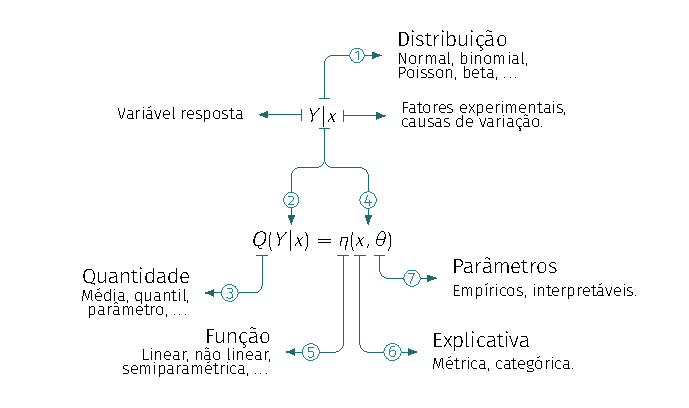
\includegraphics[width=11cm]{./img/modelos_regressao} \end{center}
\end{frame}

\begin{frame}{Modelos de regressão}
\protect\hypertarget{modelos-de-regressuxe3o-5}{}
\beginAHalfColumnT

\begin{enumerate}
\tightlist
\item
  \textbf{Definição do problema.}

  \begin{itemize}
  \tightlist
  \item
    Qual o fenômeno aleatório de interesse?
  \item
    Que fatores externos podem afetar este fenômeno?
  \end{itemize}
\item
  \textbf{Planejamento do estudo e coleta de dados.}

  \begin{itemize}
  \tightlist
  \item
    Estudo observacional x estudo experimental.
  \item
    Representação tabular.
  \end{itemize}
\end{enumerate}

\endColumns
\beginAHalfColumnT

\begin{enumerate}
\setcounter{enumi}{2}
\tightlist
\item
  \textbf{Análise dos dados via regressão.}

  \begin{itemize}
  \tightlist
  \item
    Escolha da distribuição de probabilidade.
  \item
    Especificação do modelo.
  \item
    Obtenção dos parâmetros (ajuste).
  \item
    Diagnóstico.
  \end{itemize}
\item
  \textbf{Interpretação dos resultados.}

  \begin{itemize}
  \tightlist
  \item
    Quais os fatores externos apresentam ou não impacto sobre o
    fenômeno.
  \item
    Qual a dimensão desse impacto.
  \end{itemize}
\end{enumerate}

\endColumns
\end{frame}

\begin{frame}{Modelos de regressão}
\protect\hypertarget{modelos-de-regressuxe3o-6}{}
\begin{itemize}
    \itemsep 2ex

  \item Existem modelos univariados e multivariados. 
  
    \begin{itemize}
      \item \textbf{Univariados}: apenas uma variável resposta.
      \item \textbf{Multivariados}: mais de uma variável resposta.
    \end{itemize}

  \item Em ambos os casos o interesse é avaliar o \textbf{efeito de variáveis explicativas}.
  
  \item Existem inúmeras classes de modelos de regressão, dentre elas: 
  \begin{itemize}
  \item Modelo linear normal.
  \item Modelos lineares generalizados.
  \item \textbf{Modelos multivariados de covariância linear generalizada.}
\end{itemize}

  \end{itemize}
\end{frame}

\begin{frame}{Modelo linear normal}
\protect\hypertarget{modelo-linear-normal}{}
\begin{itemize}
    \itemsep 2ex

  \item O modelo linear normal \citep{galton} ficou famoso por suas \textbf{facilidades computacionais}. 
  
  \item Possui \textbf{pressupostos} difíceis de serem atendidos na prática.
    \begin{itemize}
      \item Independência.
      \item Normalidade.
      \item Variância constante.
    \end{itemize}
  
  \item Diversas técnicas foram propostas para solucionar casos em que os pressupostos fossem violados.
  
  \end{itemize}
\end{frame}

\begin{frame}{Modelos lineares generalizados}
\protect\hypertarget{modelos-lineares-generalizados}{}
\begin{itemize}
    \itemsep 2ex

  \item O \textbf{avanço computacional} permitiu o surgimento de modelos mais gerais que necessitavam de \textbf{processos iterativos} para estimação dos parâmetros. 
  
  \item Surgem os modelos lineares generalizados(GLMs) \citep{Nelder72}. 
  
  \item Os GLMs permitem utilizar qualquer membro da \textbf{família exponencial de distribuições}.

  \item Casos especiais: Bernoulli, binomial, Poisson, normal, gama, normal inversa, entre outras.
  
  \end{itemize}
\end{frame}

\begin{frame}{Modelos multivariados de covariância linear generalizada}
\protect\hypertarget{modelos-multivariados-de-covariuxe2ncia-linear-generalizada}{}
\begin{itemize}
    \itemsep 2ex
  
  \item Apesar do grande potencial, os GLMs apresentam três importantes \textbf{restrições}:
    \begin{enumerate}
      \itemsep 2ex
    
      \item A incapacidade de lidar com \textbf{observações dependentes}. 
      \item A incapacidade de lidar com \textbf{múltiplas respostas} simultaneamente.
      \item Leque reduzido de \textbf{distribuições disponíveis}. 
    \end{enumerate}

  \item Os modelos multivariados de covariância linear generalizada (McGLMs) \citep{Bonat16} contornam estas restrições.

  \end{itemize}
\end{frame}

\begin{frame}{Modelos multivariados de covariância linear generalizada}
\protect\hypertarget{modelos-multivariados-de-covariuxe2ncia-linear-generalizada-1}{}
\begin{itemize}
   
   \itemsep 2ex
   
  \item Configuram uma estrutura geral para análise via modelos de regressão.
  
  \item Comporta múltiplas respostas de diferentes naturezas.
  
  \item Pode-se ajustar modelos com diferentes preditores e distribuições para cada resposta.
  
  \item Os modelos levam em conta a correlação entre indivíduos do conjunto de dados. 

\end{itemize}
\end{frame}

\begin{frame}{Modelos multivariados de covariância linear generalizada}
\protect\hypertarget{modelos-multivariados-de-covariuxe2ncia-linear-generalizada-2}{}
\begin{itemize}
   
   \itemsep 2ex
  
  \item Os parâmetros são interpretáveis:
  
    \begin{itemize}
    
    \itemsep 2ex
      
      \item \textbf{Parâmetros de regressão}: efeito das variáveis explicativas sobre as respostas.
      
      \item \textbf{Parâmetros de dispersão}: impacto da correlação entre unidades.
      
      \item \textbf{Parâmetros de potência}: indicativo de qual distribuição se adequa ao problema.
      
      \item \textbf{Parâmetros correlação}: força de associação entre respostas.
      
    \end{itemize}

\end{itemize}
\end{frame}

\begin{frame}{Testes de hipóteses em modelos de regressão}
\protect\hypertarget{testes-de-hipuxf3teses-em-modelos-de-regressuxe3o}{}
\begin{itemize}
    \itemsep 2ex
  
  \item Usados para verificar se a \textbf{retirada de determinada variável} explicativa do modelo geraria uma \textbf{perda no ajuste}.
  
  \item Os três testes mais usados são:

    \begin{itemize}
      \item O teste da razão de verossimilhanças \citep{trv}.
      \item O teste Wald \citep{wald}.
      \item O teste do multiplicador de lagrange ou teste escore \citep{score1,score2,score3}.
    \end{itemize}
  
  \item São baseados na função de verossimilhança dos modelos.
  
  \item São \textbf{assintóticamente equivalentes} \citep{engle}.
  
  \end{itemize}
\end{frame}

\begin{frame}{Testes de hipóteses em modelos de regressão}
\protect\hypertarget{testes-de-hipuxf3teses-em-modelos-de-regressuxe3o-1}{}
\textbf{Teste da razão de verossimilhanças}

\begin{itemize}

  \itemsep 2ex
  
  \item Efetuado a partir de dois modelos com o objetivo de compará-los. 
  \item Obter um modelo com todas as variáveis explicativas e um segundo modelo sem algumas dessas variáveis. 

  \item  O teste é usado para comparar estes modelos por meio da diferença do logaritmo da função de verossimilhança. 

\end{itemize}
\end{frame}

\begin{frame}{Testes de hipóteses em modelos de regressão}
\protect\hypertarget{testes-de-hipuxf3teses-em-modelos-de-regressuxe3o-2}{}
\textbf{Teste Wald}

\begin{itemize}

  \itemsep 2ex
  
  \item Requer apenas um modelo ajustado. 

  \item Consiste em verificar se existe evidência para afirmar que um ou mais parâmetros são iguais a valores postulados. 

  \item Avalia quão longe o valor estimado está do valor postulado. 

  \item É possível formular hipóteses para múltiplos parâmetros, 

\end{itemize}
\end{frame}

\begin{frame}{Testes de hipóteses em modelos de regressão}
\protect\hypertarget{testes-de-hipuxf3teses-em-modelos-de-regressuxe3o-3}{}
\textbf{Teste Escore}

\begin{itemize}

  \itemsep 2ex
  
  \item Requer apenas um modelo ajustado. 

  \item O modelo ajustado não possui o parâmetro de interesse

  \item O que é feito é testar se adicionar esta variável omitida resultará em uma melhora significativa no modelo. 

\end{itemize}
\end{frame}

\begin{frame}{ANOVA, MANOVA e testes de comparações múltiplas}
\protect\hypertarget{anova-manova-e-testes-de-comparauxe7uxf5es-muxfaltiplas}{}
Existe uma série de
\textbf{procedimentos baseados em testes de hipóteses}, tais como:

\begin{itemize}

  \itemsep 2ex
  
  \item Análise de variância (ANOVA).
  \item Análise de variância multivariada (MANOVA).
  \item Testes de comparações múltiplas.

\end{itemize}
\end{frame}

\begin{frame}{ANOVA \& MANOVA}
\protect\hypertarget{anova-manova}{}
\begin{itemize}
    \itemsep 2ex

  \item Formas de \textbf{avaliar a significância} de cada uma das variáveis de uma forma procedural.  
  
  \item Consiste em efetuar testes sucessivos impondo \textbf{restrições ao modelo} original. 

  \item O objetivo é testar se a ausência de determinada variável gera perda ao modelo. 

  \item Os resultados são sumarizados numa tabela, o chamado \textbf{quadro de análise de variância}.

  \item Caso univariado: ANOVA \citep{anova_fisher}. Caso multivariado: MANOVA \citep{manova}.
  
  \end{itemize}
\end{frame}

\begin{frame}{Testes de comparações múltiplas}
\protect\hypertarget{testes-de-comparauxe7uxf5es-muxfaltiplas}{}
\begin{itemize}
  \itemsep 2ex
    
  \item Complementar às ANOVAs e MANOVAs

  \item São utilizados quando a análise de variância aponta como conclusão a existência de efeito significativo dos parâmetros associados a uma variável categórica.

  \item A análise de variância mostrará se há efeito de uma variável no modelo.
 
  \item Os testes de comparações múltiplas determinam \textbf{quais níveis diferem entre si}. 

\end{itemize}
\end{frame}

\begin{frame}{Temas abordados até aqui}
\protect\hypertarget{temas-abordados-atuxe9-aqui}{}
\begin{itemize}
  \itemsep 2ex
    
  \item Ciência de dados.

  \item Modelos de regressão.

  \item Classes de modelos de regressão (ênfase nos \textbf{McGLMs}).

  \item Testes de hipóteses em modelos de regressão (ênfase no \textbf{teste Wald}).

  \item Procedimentos baseados em testes de hipóteses (ANOVA, MANOVA, testes de comparações múltiplas).

\end{itemize}
\end{frame}

\begin{frame}{Desafio e hipótese}
\protect\hypertarget{desafio-e-hipuxf3tese}{}
\begin{itemize}
  \itemsep 2ex
    
  \item Não há discussão a respeito da construção de testes de hipóteses para os McGLMs.

  \item Contudo, os McGLMs apresentam os elementos necessários para utilizar o teste Wald:
    \begin{enumerate}
      \item Um vetor de estimativas dos parâmetros
      \item Uma matriz de variância e covariância destas estimativas.
    \end{enumerate}
    
  \item Das três opções clássicas de testes de hipóteses, o teste Wald se torna o mais atrativo para os McGLMs. 

\end{itemize}
\end{frame}

\begin{frame}{Objetivo}
\protect\hypertarget{objetivo}{}
\begin{enumerate}
  \itemsep 2ex
  
 \item Propor a utilização do teste Wald para realização de testes de hipóteses gerais sobre parâmetros de regressão e dispersão de McGLMs.

 \item Avaliar as propriedades e comportamento dos testes propostos com base em estudos de simulação.
 
 \item Implementar funções em R para testes de hipóteses, ANOVA, MANOVA e testes de comparações múltiplas para os McGLMs. 
 
 \item Motivar o potencial de aplicação das metodologias discutidas com base na aplicação a conjuntos de dados reais.

\end{enumerate}
\end{frame}

\begin{frame}{Contribuição}
\protect\hypertarget{contribuiuxe7uxe3o}{}
\begin{itemize}
  \itemsep 2ex
  
  \item Formas de avaliar os parâmetros estimados pelos McGLMs.

  \item Fornecer ferramentas para uma melhor interpretação dos parâmetros estimados.
 
  \item Fornecer uma maneira procedural e segura de responder questões comuns no contexto de modelagem.
 
  \item Extrair mais informações e conclusões a respeito dos problemas modelados por meio dos McGLMs.

\end{itemize}
\end{frame}

\hypertarget{referencial-teuxf3rico}{%
\section{Referencial teórico}\label{referencial-teuxf3rico}}

\begin{frame}{Referencial teórico}
\begin{enumerate}
    \itemsep 2ex
    
  \item McGLMs
    \begin{itemize}
      \item Elementos.
      \item Preditores lineares e matriciais.
      \item Funções de variância.
      \item Parâmetros.
      \item Estimação.
    \end{itemize}
    
  \item Testes de hipóteses
    \begin{itemize}
      \item Elementos de um teste de hipóteses.
      \item Testes de hipóteses em modelos de regressão.
      \item Teste Wald
      \item ANOVA e MANOVA.
      \item Testes de comparações múltiplas.
    \end{itemize}
\end{enumerate}
\end{frame}

\hypertarget{modelos-multivariados-de-covariuxe2ncia-linear-generalizada-3}{%
\section{Modelos multivariados de covariância linear
generalizada}\label{modelos-multivariados-de-covariuxe2ncia-linear-generalizada-3}}

\begin{frame}{Modelos multivariados de covariância linear generalizada}
\end{frame}

\begin{frame}{Modelos multivariados de covariância linear generalizada}
\protect\hypertarget{modelos-multivariados-de-covariuxe2ncia-linear-generalizada-4}{}
Para definição de um McGLM considere:

\begin{itemize}
  
  \itemsep 2ex
  
  \item $\boldsymbol{Y}_{N \times R} = \left \{ \boldsymbol{Y}_1, \dots, \boldsymbol{Y}_R \right \}$ uma  matriz de variáveis resposta.
  
  \item $\boldsymbol{M}_{N \times R} = \left \{ \boldsymbol{\mu}_1, \dots, \boldsymbol{\mu}_R \right \}$ uma matriz de valores esperados.
  
    \item $\boldsymbol{X}_r$ denota uma matriz de delineamento $N \times k_r$.
  
  \item $\boldsymbol{\beta}_r$ denota um vetor $k_r \times 1$ de parâmetros de regressão.
  
\end{itemize}
\end{frame}

\begin{frame}{Modelos multivariados de covariância linear generalizada}
\protect\hypertarget{modelos-multivariados-de-covariuxe2ncia-linear-generalizada-5}{}
Considere ainda:

\begin{itemize}
  
  \itemsep 2ex
  
    \item $\Sigma_b$ uma matriz de correlação entre variáveis resposta, de ordem $R \times R$.
    
  \item $\Sigma_r$, $r = 1,..., R$, a matriz de variância e covariância para cada resposta $r$, de dimensão $NxN$:
  
$$
\Sigma_r = \mathrm{V}_r\left(\boldsymbol{\mu}_r; p_r\right)^{1/2}(\boldsymbol{\Omega}\left(\boldsymbol{\tau}_r\right))\mathrm{V}_r\left(\boldsymbol{\mu}_r; p_r\right)^{1/2}.
$$

Em que:

  \begin{itemize}
    \item $\mathrm{V}_r\left(\boldsymbol{\mu}; p\right)$ é uma matriz diagonal em que as entradas principais são dadas pela função de variância aplicada ao vetor $\boldsymbol{\mu}$. 
  
  \item $p_r$ é o parâmetro de potência. 
  
  \item $\boldsymbol{\Omega}\left(\boldsymbol{\tau}_r\right)$ a matriz de dispersão que descreve a parte da covariância dentro de cada variável resposta. 
  \end{itemize}
  
\end{itemize}
\end{frame}

\begin{frame}{Preditor linear matricial}
\protect\hypertarget{preditor-linear-matricial}{}
\begin{itemize}
  
  \itemsep 2ex
  
  \item A matriz $\boldsymbol{\Omega}(\boldsymbol{\tau}_r)$ descreve a estrutura de correlação entre as observações da amostra.
  
  \item É modelada através de um preditor linear matricial combinado com uma função de ligação de covariância:

$$
h\left \{ \boldsymbol{\Omega}(\boldsymbol{\tau}_r) \right \} = \tau_{r0}Z_0 + \ldots + \tau_{rD}Z_D
$$
  
  \begin{itemize}
  
  \itemsep 2ex
  
  \item $h()$ é a função de ligação de covariância.
  
  \item $Z_{rd}$ com $d$ = 0,$\ldots$, D são matrizes que representam a estrutura de covariância presente em cada variável resposta $r$.
  
  \item $\boldsymbol{\tau_r}$ = $(\tau_{r0}, \ldots, \tau_{rD})$ é um vetor $(D + 1) \times 1$ de parâmetros de dispersão. 
  
\end{itemize}

\end{itemize}
\end{frame}

\begin{frame}{Funções de variância}
\protect\hypertarget{funuxe7uxf5es-de-variuxe2ncia}{}
\begin{enumerate}
  \item \textbf{Função de variância potência} \citep{Jorgensen87, Jorgensen97}.
  
    \begin{itemize}
      \item Família Tweedie de distribuições.
      \item $\vartheta\left(\boldsymbol{\mu}; p\right) = \mu^p$.
      \item Casos particulares: normal ($p$ = 0), Poisson ($p$ = 1), gama ($p$ = 2) e normal inversa ($p$ = 3).
    \end{itemize}

  
  \item \textbf{Função de dispersão Poisson–Tweedie} \citep{Jorgensen15}.
  
    \begin{itemize}
      \item Família Poisson-Tweedie de distribuições.
      \item $\vartheta\left(\boldsymbol{\mu}; p\right) = \mu + \mu^p$.
      \item Casos particulares: Hermite ($p$ = 0), Neyman tipo A ($p$ = 1), binomial negativa ($p$ = 2) e Poisson–inversa gaussiana (p = $3$).
      
    \end{itemize}

  \item \textbf{Função de variância binomial.} 
  
    \begin{itemize}
      \item $\vartheta(\boldsymbol{\mu}) = \mu(1 - \mu)$.
      \item Acomoda respostas binárias ou restritas a um intervalo.
    \end{itemize}

\end{enumerate}
\end{frame}

\begin{frame}{Modelos multivariados de covariância linear
generalizada\}}
\protect\hypertarget{modelos-multivariados-de-covariuxe2ncia-linear-generalizada-6}{}
Os McGLMs são definidos por:

\begin{center}
$\mathrm{E}(\boldsymbol{Y}) = \boldsymbol{M} = \{g_1^{-1}(\boldsymbol{X}_1 \boldsymbol{\beta}_1), \ldots, g_R^{-1}(\boldsymbol{X}_R \boldsymbol{\beta}_R)\}$

$\mathrm{Var}(\boldsymbol{Y}) = \boldsymbol{C} = \boldsymbol{\Sigma}_R \overset{G} \otimes \boldsymbol{\Sigma}_b$

\end{center}

Em que:

\begin{itemize}
  
  \item $\boldsymbol{\Sigma}_R \overset{G} \otimes \boldsymbol{\Sigma}_b = \mathrm{Bdiag}(\tilde{\boldsymbol{\Sigma}}_1, \ldots, \tilde{\boldsymbol{\Sigma}}_R) (\boldsymbol{\Sigma}_b \otimes \boldsymbol{I}) \mathrm{Bdiag}(\tilde{\boldsymbol{\Sigma}}_1^\top, \ldots, \tilde{\boldsymbol{\Sigma}}_R^\top)$ é o produto generalizado de Kronecker.
  
  \item $\tilde{\boldsymbol{\Sigma}}_r$ denota a matriz triangular inferior da decomposição de Cholesky da matriz ${\boldsymbol{\Sigma}}_r$.
  
  \item $\mathrm{Bdiag()}$ denota a matriz bloco-diagonal.
  
  \item $\boldsymbol{I}$ uma matriz identidade $N \times N$.
  
  \item $g_r()$ são as tradicionais funções de ligação.
  
\end{itemize}
\end{frame}

\begin{frame}{Modelos multivariados de covariância linear generalizada}
\protect\hypertarget{modelos-multivariados-de-covariuxe2ncia-linear-generalizada-7}{}
\begin{itemize}

\itemsep 2ex
  
  \item Parâmetros estimados nos McGLMs:
    \begin{enumerate}
      \item Regressão.
      \item Dispersão.
      \item Potência.
      \item Correlação.
    \end{enumerate}
  
  \item Todas estas quantidades são interpretáveis e são estimadas com base nos dados.
  
  \item A estimação é feita por meio de \textbf{funções de estimação}.
    \begin{enumerate}
      \item \textbf{Função quasi-score} para parâmetros de regressão. 
      \item \textbf{Função de estimação de Pearson} para os demais parâmetros. 
    \end{enumerate}

\end{itemize}
\end{frame}

\begin{frame}{Funções de estimação}
\protect\hypertarget{funuxe7uxf5es-de-estimauxe7uxe3o}{}
\begin{center}
$\psi_{\boldsymbol{\beta}}(\boldsymbol{\beta}, \boldsymbol{\lambda}) = \boldsymbol{D}^\top \boldsymbol{C}^{-1}(\mathcal{Y} - \mathcal{M})$

$\psi_{\boldsymbol{\lambda}_i}(\boldsymbol{\beta}, \boldsymbol{\lambda}) = \mathrm{tr}(W_{\boldsymbol{\lambda}i} (\boldsymbol{r}^\top\boldsymbol{r} - \boldsymbol{C})),  i = 1,.., Q$
\end{center}

Em que:

\begin{itemize}
  
  \item \normalsize $\boldsymbol{\beta}_r$ denota um vetor $k_r \times 1$ de parâmetros de regressão.
  
  \item \normalsize $\boldsymbol{\lambda}$ é um vetor $Q \times 1$ de parâmetros de dispersão.
  
  \item \normalsize $\mathcal{Y}$ é um vetor $NR \times 1$ com os valores da matriz de variáveis respostas $Y_{N \times R}$ empilhados.
  
  \item \normalsize $\mathcal{M}$ é um vetor $NR \times 1$ com os valores da matriz de valores esperados $M_{N \times R}$ empilhados.
  
  \item \normalsize $\boldsymbol{D} = \nabla_{\boldsymbol{\beta}} \mathcal{M}$ 
é uma matriz $NR \times K$, e $\nabla_{\boldsymbol{\beta}}$ denota o 
operador gradiente.
  
  \item \normalsize $W_{\boldsymbol{\lambda}i} = -\frac{\partial
    \boldsymbol{C}^{-1}}{\partial \boldsymbol{\lambda}_i}$ 
    
  \item \normalsize $\boldsymbol{r} = (\mathcal{Y} - \mathcal{M})$
  
\end{itemize}
\end{frame}

\begin{frame}{Distribuição assintótica e algoritmo de estimação}
\protect\hypertarget{distribuiuxe7uxe3o-assintuxf3tica-e-algoritmo-de-estimauxe7uxe3o}{}
\begin{itemize}

  \item Para resolver o sistema de equações $\psi_{\boldsymbol{\beta}} = 0$ e $\psi_{\boldsymbol{\lambda}} = 0$ faz-se uso do algoritmo Chaser modificado:

$$
\begin{matrix}
\boldsymbol{\beta}^{(i+1)} = \boldsymbol{\beta}^{(i)}- S_{\boldsymbol{\beta}}^{-1} \psi \boldsymbol{\beta} (\boldsymbol{\beta}^{(i)}, \boldsymbol{\lambda}^{(i)}), \\ 
\boldsymbol{\lambda}^{(i+1)} = \boldsymbol{\lambda}^{(i)}\alpha S_{\boldsymbol{\lambda}}^{-1} \psi \boldsymbol{\lambda} (\boldsymbol{\beta}^{(i+1)}, \boldsymbol{\lambda}^{(i)}).
\end{matrix}
$$

  \item Seja $\boldsymbol{\hat{\theta}} = (\boldsymbol{\hat{\beta}^{\top}}, \boldsymbol{\hat{\lambda}^{\top}})^{\top}$ o estimador baseado em funções de estimação de $\boldsymbol{\theta}$.
  
  \item A distribuição assintótica de $\boldsymbol{\hat{\theta}}$ é:

$$
\boldsymbol{\hat{\theta}} \sim N(\boldsymbol{\theta}, J_{\boldsymbol{\theta}}^{-1}),
$$

\noindent $J_{\boldsymbol{\theta}}^{-1}$ é a inversa da matriz de informação de Godambe, dada por
  
$$J_{\boldsymbol{\theta}}^{-1} = S_{\boldsymbol{\theta}}^{-1} V_{\boldsymbol{\theta}} S_{\boldsymbol{\theta}}^{-\top},$$ 

\noindent em que $S_{\boldsymbol{\theta}}^{-\top} = (S_{\boldsymbol{\theta}}^{-1})^{\top}.$

\end{itemize}
\end{frame}

\hypertarget{testes-de-hipuxf3teses}{%
\section{Testes de hipóteses}\label{testes-de-hipuxf3teses}}

\begin{frame}{Testes de hipóteses}
\end{frame}

\begin{frame}{Testes de hipóteses}
\protect\hypertarget{testes-de-hipuxf3teses-1}{}
\begin{itemize}
    \itemsep 2ex
  
  \item Inferência: \textbf{inferir} conclusões válidas a respeito de uma população por meio do estudo de uma amostra.
  
  \item Problemas de inferência estatística são:
    \begin{enumerate}
    
      \itemsep 2ex
      
      \item \textbf{Estimação} de parâmetros com base em informação amostral.
      
      \item \textbf{Testes de hipóteses}.
        \begin{itemize}
          \item Com base na evidência amostral, podemos considerar que dado parâmetro tem determinado valor?
        \end{itemize}
    
    \end{enumerate}
  
  \end{itemize}
\end{frame}

\begin{frame}{Testes de hipóteses}
\protect\hypertarget{testes-de-hipuxf3teses-2}{}
\begin{itemize}
    \itemsep 2ex
  
  \item São postuladas 2 hipóteses, chamadas de \textbf{nula} e \textbf{alternativa}.
  
  \item Avalia-se uma estatística de teste. 
  
  \item Com base no valor da estatística e de acordo com sua distribuição de probabilidade, toma-se a decisão de rejeitar ou não rejeitar a hipótese nula.
    
  \item Seja $\theta$ um parâmetro, um teste de hipóteses sobre $\theta$ é dado por:
  
$$
\left\{\begin{matrix}
H_0: \theta = \theta_0 \\ 
H_1: \theta \neq \theta_0
\end{matrix}\right.
$$  
  
  \end{itemize}
\end{frame}

\begin{frame}{Testes de hipóteses}
\protect\hypertarget{testes-de-hipuxf3teses-3}{}
Desfechos possíveis:

\begin{table}[]
\begin{tabular}{l|cc}
\hline
\multicolumn{1}{c|}{}    & \textbf{Rejeita $H_0$} & \textbf{Não Rejeita $H_0$} \\ \hline
\textbf{$H_0$ verdadeira} & Erro tipo I           & Decisão correta           \\
\textbf{$H_0$ falsa}      & Decisão correta       & Erro tipo II              \\ \hline
\end{tabular}
\caption{Desfechos possíveis em um teste de hipóteses}
\label{tab:my-table}
\end{table}

\begin{itemize}
    \itemsep 2ex
  
  \item A probabilidade do erro do tipo I recebe o nome de nível de significância.
  
  \item A probabilidade de se rejeitar corretamente $H_0$ recebe o nome de poder do teste.
  
  \item A probabilidade de a estatística de teste tomar um valor igual ou mais extremo do que aquele que foi observado recebe o nome de valor-p.
    
  \end{itemize}
\end{frame}

\begin{frame}{Testes de hipóteses em modelos de regressão}
\protect\hypertarget{testes-de-hipuxf3teses-em-modelos-de-regressuxe3o-4}{}
\begin{itemize}
  \itemsep 2ex

  \item Modelos de regressão: modelar uma ou mais variáveis em função de um conjunto de variáveis explicativas. 

  \item Modelos contêm parâmetros que são quantidades desconhecidas que estabelecem a relação entre as variáveis sob o modelo. 

  \item Pode ser de interesse verificar se a retirada de uma ou mais variáveis do modelo gera um modelo significativamente pior que o original. 

  \item Verificar se há evidência suficiente nos dados para afirmar que determinada variável explicativa não possui efeito sobre a resposta.

\end{itemize}
\end{frame}

\begin{frame}{Teste Wald em modelos de regressão}
\protect\hypertarget{teste-wald-em-modelos-de-regressuxe3o}{}
\begin{itemize}
  \itemsep 2ex

  \item A ideia do teste consiste em verificar se existe evidência suficiente nos dados para afirmar que um ou mais parâmetros são iguais a valores especificados.
  
  \item Avalia a distância entre as estimativas dos parâmetros e um conjunto de valores postulados.
  
  \item Esta diferença é ainda padronizada por medidas de precisão das estimativas dos parâmetros. 

  \item Quanto maior for esta distância padronizada, menores são as evidências a favor da hipótese de que os valores estimados são iguais aos valores postulados.


  \end{itemize}
\end{frame}

\begin{frame}{Teste Wald em modelos de regressão}
\protect\hypertarget{teste-wald-em-modelos-de-regressuxe3o-1}{}
Considere um modelo de regressão em que:

\begin{itemize}

  \itemsep 2ex
  
  \item $\boldsymbol{\beta}$ um vetor $k\times1$ parâmetros de regressão.
    
  \item $\boldsymbol{\hat\beta}$ as estimativas dos parâmetros.
    
  \item $\boldsymbol{c}$ um vetor de valores postulados de dimensão $s$.
    
  \item $\boldsymbol{L}$ uma matriz de especificação das hipóteses, de dimensão $s \times k$.  
    
  \end{itemize}
\end{frame}

\begin{frame}{Teste Wald em modelos de regressão}
\protect\hypertarget{teste-wald-em-modelos-de-regressuxe3o-2}{}
\begin{itemize}

  \itemsep 2ex
  
  \item As hipóteses podem ser descritas como:

$$
\left\{\begin{matrix}
H_0: \boldsymbol{L}\boldsymbol{\beta} = \boldsymbol{c} \\ 
H_1: \boldsymbol{L}\boldsymbol{\beta} \neq \boldsymbol{c}
\end{matrix}\right.
$$

  \item A estatística de teste é dada por:

$$
WT = (\boldsymbol{L\hat\beta} - \boldsymbol{c})^T \ (\boldsymbol{L \ Var^{-1}(\hat\beta) \ L^T})^{-1} \ (\boldsymbol{L\hat\beta} - \boldsymbol{c}).
$$

 \item  WT $\sim \chi^2_s$.

\end{itemize}
\end{frame}

\begin{frame}{ANOVA e MANOVA}
\protect\hypertarget{anova-e-manova}{}
\begin{itemize}

  \itemsep 2ex

  \item Testes sucessivos impondo restrições ao modelo original. 

  \item O objetivo é testar se a ausência de determinada variável gera um modelo significativamente inferior. 

  \item O quadro de ANOVA ou MANOVA contém em cada linha: 
    \begin{enumerate}
      \item A variável. 
      \item O valor de uma estatística de teste referente à hipótese de nulidade de todos os parâmetros associados a esta variável. 
      \item Os graus de liberdade desta hipótese. 
      \item Um valor-p associado à hipótese testada naquela linha do quadro.
    \end{enumerate}

  \item É possível gerar quadros de análise de variância por meio do teste Wald.

  \end{itemize}
\end{frame}

\begin{frame}{Testes de comparações múltiplas}
\protect\hypertarget{testes-de-comparauxe7uxf5es-muxfaltiplas-1}{}
\begin{itemize}

  \itemsep 2ex

  \item Usado quando a ANOVA aponta para efeito significativo de uma variável categórica.

  \item Comparações aos pares a fim de detectar para quais níveis da variável categórica os valores da resposta se alteram.

  \item Pode ser avaliada utilizando o teste Wald. 

  \item Por meio da correta especificação da matriz $\boldsymbol{L}$, é possível avaliar hipóteses sobre qualquer possível contraste entre os níveis de uma determinada variável categórica. 

\end{itemize}
\end{frame}

\hypertarget{trabalhos-relacionados}{%
\section{Trabalhos relacionados}\label{trabalhos-relacionados}}

\begin{frame}{Trabalhos relacionados}
\end{frame}

\begin{frame}{Trabalhos relacionados}
\protect\hypertarget{trabalhos-relacionados-1}{}
\begin{itemize}
  \itemsep 2ex
  
  \item Propostas que visam contornar restrições dos GLMs e como são efetuados testes de hipóteses para estas propostas.
  
  \item Propostas univariadas e multivariadas.
  
  \item Efeitos aleatórios.
  
  \item Correção de erros padrões.
  
  \item Grande variedade de modelos de regressão multivariados para fins específicos.
  
\end{itemize}
\end{frame}

\begin{frame}{Trabalhos relacionados}
\protect\hypertarget{trabalhos-relacionados-2}{}
\begin{itemize}
  \itemsep 2ex
  
  \item Efeitos aleatórios para acomodar correlação entre observações.

  \item Modelos lineares generalizados mistos (GLMM). Modelos lineares generalizados multivariados mistos (MGLMM).
  
 \item A interpretação dos parâmetros de regressão dependem de manter o efeito aleatório fixado.
 
 \item A estimação destes modelos não é simples. Envolve integrais complexas e é uma tarefa computacionalmente desafiadora.

 \item É possível usar máxima verossimilhança. 
 
 \item Testes de hipóteses tradicionais costumam ser empregados.
  
\end{itemize}
\end{frame}

\begin{frame}{Trabalhos relacionados}
\protect\hypertarget{trabalhos-relacionados-3}{}
\begin{itemize}
  \itemsep 2ex
  
  \item Equações de estimação generalizadas (GEE).

  \item Alternativa para acomodar a correlação entre observações. 
 
  \item Incluir no processo de estimação uma matriz de correlação de trabalho. 
 
  \item O foco do método não é a modelagem da estrutura de correlação entre os indivíduos, mas sim a correção dos erros padrões.
 
  \item Testes de hipóteses tradicionais costumam ser empregados.
  
\end{itemize}
\end{frame}

\begin{frame}{Trabalhos relacionados}
\protect\hypertarget{trabalhos-relacionados-4}{}
\begin{itemize}
  \itemsep 2ex
  
  \item Modelos aditivos generalizados para locação, escala e forma (GAMLSS). 
 
  \item Classe de modelos de regressão univariados com um número considerável de distribuições disponíveis. 
 
  \item É possível modelar todos os parâmetros distribucionais.
 
  \item É possível incluir efeitos aleatórios e termos suavizadores. 
 
  \item A estimação é feita com base verossimilhança penalizada.
 
  \item Testes de hipóteses tradicionais costumam ser empregados.
 
\end{itemize}
\end{frame}

\begin{frame}{Trabalhos relacionados}
\protect\hypertarget{trabalhos-relacionados-5}{}
Grande variedade de modelos de regressão multivariados para fins
específicos.

\begin{itemize}
  \itemsep 2ex
  
  \item Análise de contagens multivariadas em que os testes usuais se aplicam \citep{zhang2017regression}.  

  \item Modelo de regressão multivariado com distribuição Poisson inversa gaussiana em que testes de hipóteses ao estilo da razão de verossimilhanças se aplicam \citep{mardalena2020parameter}. 

  \item Modelo de regressão Poisson zero inflacionado multivariado em que o teste da razão de verossimilhanças e o teste Wald se aplicam \citep{sari2021estimation}.
  
  \item Modelo de regressão multivariado gamma em que um análogo do teste da razão de verossimilhanças e o teste Wald se aplicam \citet{rahayu2020multivariate}.

\end{itemize}
\end{frame}

\hypertarget{teste-wald-para-mcglms}{%
\section{Teste Wald para McGLMs}\label{teste-wald-para-mcglms}}

\begin{frame}{Teste Wald para McGLMs}
\begin{enumerate}
  \itemsep 2ex
    
  \item Definição das hipóteses.
  \item Estatística de teste.
  \item Distribuição.
  \item Hipóteses comuns.
  \item Construção da matriz $\boldsymbol{L}$.
  \item Exemplos.
  
\end{enumerate}
\end{frame}

\begin{frame}{Hipóteses}
\protect\hypertarget{hipuxf3teses}{}
\[H_0: \boldsymbol{L}\boldsymbol{\theta^{*}} = \boldsymbol{c} \ vs \ H_1: \boldsymbol{L}\boldsymbol{\theta^{*}} \neq \boldsymbol{c}.\]

Em que:

\begin{itemize}
  
  \item $\boldsymbol{\theta^{*}}$ é o vetor de dimensão $h \times 1$ de parâmetros de regressão, dispersão e potência do modelo. 
  
  \item Em que $\boldsymbol{L}$ é a matriz de especificação das hipóteses a serem testadas, tem dimensão $s \times h$. 
  
  \item $\boldsymbol{c}$ é um vetor de dimensão $s \times 1$ com os valores sob hipótese nula.

\end{itemize}
\end{frame}

\begin{frame}{Estatística de teste}
\protect\hypertarget{estatuxedstica-de-teste}{}
\[W = (\boldsymbol{L\hat\theta^{*}} - \boldsymbol{c})^T \ (\boldsymbol{L \ J^{\boldsymbol{*}-1} \ L^T})^{-1} \ (\boldsymbol{L\hat\theta^{*}} - \boldsymbol{c}).\]

Em que:

\begin{itemize}
  \item $\boldsymbol{L}$ é a matriz da especificação das hipóteses, tem dimensão $s \times h$. 

  \item $\boldsymbol{\hat\theta^{*}}$ é o vetor de dimensão $h \times 1$ com todas as estimativas dos parâmetros de regressão, dispersão e potência. 

  \item $\boldsymbol{c}$ é um vetor de dimensão $s \times 1$ com os valores sob hipótese nula. 

  \item E $\boldsymbol{J^{\boldsymbol{*}-1}}$ é a inversa da matriz de informação de Godambe desconsiderando os parâmetros de correlação, de dimensão $h \times h$. 
  
  \item $W \sim \chi^2_s$

\end{itemize}
\end{frame}

\begin{frame}{Hipóteses comuns}
\protect\hypertarget{hipuxf3teses-comuns}{}
\begin{itemize}
  \itemsep 2ex
  
  \item Costuma ser de interesse formular:
    \begin{enumerate}
      \itemsep 2ex
      \item Hipóteses para parâmetros individuais.
      \item Hipóteses para múltiplos parâmetros.
      \item Hipóteses para avaliar igualdade de parâmetros
      \item Hipóteses sobre parâmetros de regressão ou dispersão para respostas sob mesmo preditor.
      \item Hipóteses sobre contrastes.
\end{enumerate}
  
  \item O elemento chave é a correta especificação da matriz $\boldsymbol{L}$.
  
\end{itemize}
\end{frame}

\begin{frame}{Construção da matriz \(\boldsymbol{L}\)}
\protect\hypertarget{construuxe7uxe3o-da-matriz-boldsymboll}{}
\begin{itemize}
  \itemsep 2ex
  
  \item Cada coluna da matriz $\boldsymbol{L}$ corresponde a um dos $h$ parâmetros de $\boldsymbol{\theta^{*}}$. 
  
  \item Cada linha corresponde a uma restrição. 

  \item A matriz é composta por valores iguais a 0, 1 e eventualmente -1.
  
  \item O produto $\boldsymbol{L}\boldsymbol{\theta^{*}}$ deve resultar nas hipóteses de interesse.

\end{itemize}
\end{frame}

\hypertarget{exemplo-seuxe7uxe3o}{%
\section{Exemplo seção}\label{exemplo-seuxe7uxe3o}}

\begin{frame}{Exemplo subseção}
\protect\hypertarget{exemplo-subseuxe7uxe3o}{}
\begin{itemize}
\tightlist
\item
  bullet.
\end{itemize}
\end{frame}

\begin{frame}{Exemplo figura}
\protect\hypertarget{exemplo-figura}{}
\begin{center}
\includegraphics[width=0.8\linewidth]{./img/Cursos} \end{center}
\end{frame}

\hypertarget{outra-seuxe7uxe3o}{%
\section{Outra seção}\label{outra-seuxe7uxe3o}}

\begin{frame}[fragile]{Exemplo slide 2 colunas}
\protect\hypertarget{exemplo-slide-2-colunas}{}
\beginAHalfColumnT

\begin{itemize}
\tightlist
\item
  \texttt{R} para data science.

  \begin{itemize}
  \tightlist
  \item
    Data: 04 a 15/05/2021.
  \item
    \textbf{Consulte condições de acesso.}
  \end{itemize}
\item
  Matemática para data science.

  \begin{itemize}
  \tightlist
  \item
    Data: 01 a 12/05/2021.
  \end{itemize}
\item
  Probabilidade e Estatística para data science.

  \begin{itemize}
  \tightlist
  \item
    Data: 22/06 a 01/07/2021.
  \end{itemize}
\item
  Visualização, dashboards e relatórios dinâmicos.

  \begin{itemize}
  \tightlist
  \item
    Data: 06 a 17/07/2021.
  \end{itemize}
\end{itemize}

\endColumns
\beginAHalfColumnT

\begin{itemize}
\tightlist
\item
  Modelagem estatística para data science.

  \begin{itemize}
  \tightlist
  \item
    Data: 03 a 14/08/2021.
  \end{itemize}
\item
  Planejamento de experimentos.

  \begin{itemize}
  \tightlist
  \item
    Data: 07 a 18/09/2021.
  \end{itemize}
\item
  Cursos previstos

  \begin{itemize}
  \tightlist
  \item
    Machine learning com R.
  \item
    Mineração de texto com R.
  \item
    Web Scraping com R.
  \item
    R avançado.
  \item
    R para big data (spark).
  \end{itemize}
\end{itemize}

\endColumns
\end{frame}

\begin{frame}{Exemplo texto e figura 2 colunas}
\protect\hypertarget{exemplo-texto-e-figura-2-colunas}{}
\beginAHalfColumn

\begin{itemize}
\tightlist
\item
  A Ômega Data Science é um projeto que objetiva construir, capacitar e
  conectar pessoas em uma comunidade focada em Data Science.
\item
  Instagram:
  \href{https://instagram.com/omegadatascience}{@omegadatascience}
\item
  Twitter: \href{https://twitter.com/omegadatascienc}{@omegadatascienc}
\item
  Telegram: \textless cutt.ly/omega\_grupo\_telegram\textgreater.
\item
  YouTube:
  \href{https://youtube.com/OmegaDataScience}{/OmegaDataScience}
\end{itemize}

\endColumns
\beginAHalfColumn

\begin{center}
\includegraphics[width=0.9\linewidth]{./img/omega-quadrado-sombra} \end{center}

\endColumns
\end{frame}

\begin{frame}[allowframebreaks]{}
  \bibliographytrue
  \bibliography{config/referencias.bib}
\end{frame}

\end{document}
